\documentclass[conference]{IEEEtran}

\usepackage{cite}
\usepackage{amsmath}
\usepackage{booktabs}
\usepackage{array}
\usepackage{xcolor}
\usepackage{tikz}
\usetikzlibrary{arrows.meta,positioning,fit,backgrounds,calc}
\usepackage{algorithm}
\usepackage[noend]{algpseudocode}
\usepackage[hidelinks]{hyperref}
\usepackage{url}

\newcommand{\cn}[1]{\texttt{#1}}   % condition / code names

\begin{document}

\title{Reducing and Structuring Alive2 Counterexamples for Language-Model-Assisted Repair of LLVM Miscompilations}

\author{%
\IEEEauthorblockN{Abhyuday Vaish}
\IEEEauthorblockA{Vellore Institute of Technology Chennai\\
\texttt{abhyuday.vaish2024@vitstudent.ac.in}}
\and
\IEEEauthorblockN{Bhuvan Nayak}
\IEEEauthorblockA{Vellore Institute of Technology Chennai\\
\texttt{bhuvan.bharatnayak2024@vitstudent.ac.in}}
\and
\IEEEauthorblockN{Siddharth Sameer Nevgi}
\IEEEauthorblockA{Vellore Institute of Technology Chennai\\
\texttt{siddharth.sameer2024@vitstudent.ac.in}}
\and
\IEEEauthorblockN{Tanish Desai}
\IEEEauthorblockA{Vellore Institute of Technology Chennai\\
\texttt{tanish.somashekhar2024@vitstudent.ac.in}}
}

\maketitle

\begin{abstract}
Alive2 can report a concrete counterexample when an LLVM optimization fails refinement. Its output contains the reproducer, intermediate values, and verifier diagnostics, which a repair model must interpret while editing the compiler's C++ implementation. We study whether reducing this witness and presenting it in a fixed structure help repair. Our feedback layer crosses four reduction choices with two presentation choices, alongside a no-counterexample baseline. The IR-aware reducer edits source and target together, closes candidates over dependencies, uses seeds from the verifier report, and checks accepted changes with Alive2. The planned evaluation uses 24 stratified single-function miscompilations, three trials per bug and condition, and at most four repair turns with Qwen3-Coder-30B-A3B-Instruct. This draft reports an interim snapshot of 205 runs. Seven bugs have all three trials under all nine conditions; across them, raw structured feedback repairs two bugs, IR-aware plain feedback repairs one, and IR-aware structured feedback repairs none. These data do not establish an improvement from IR-aware reduction. The audit also identifies incomplete replacement replies, compilation failures, and unreduced witnesses that limit the comparison. We report these observations separately from a revised harness planned for further evaluation.
\end{abstract}

\begin{IEEEkeywords}
compiler testing, translation validation, Alive2, counterexample reduction, program repair, large language models, LLVM
\end{IEEEkeywords}

%=====================================================================
\section{Introduction}
%=====================================================================

When an LLVM middle-end pass miscompiles a function, Alive2 can often demonstrate the error. Given the IR before and after the pass, it searches for an input on which the target does not refine the source, and it reports that input together with the values computed by both sides~\cite{lopes2021alive2}. The repair loop of \emph{llvm-apr-benchmark} returns this report to the model after a failed patch~\cite{zheng2025aprbench}. The report is verbose relative to the information it conveys. It repeats the reproducer pair (the reproducer alone is 6 to 164 lines in the sample used here) and lists every value computed along the failing execution, most of which are unrelated to the violated refinement.

Two lines of work suggest that the form of failure feedback matters. For the repair of ordinary programs, shortening a large failure-inducing test input before it enters the prompt has been reported to help~\cite{yang2026reducefix}, as has selecting the smallest failing counterexample from a pool~\cite{he2026pgs}. For compilers, recent work studies benchmarks and agent harnesses and reports low resolution rates on LLVM bugs~\cite{zheng2026harness,tian2026llvmbench}. These settings differ from ours: the feedback here is a \emph{verifier witness for an IR transformation}, while the artifact to repair is the \emph{C++ implementation of the pass}. We ask whether a witness reduced with IR structure and presented in labelled sections helps more than raw feedback. The interim evidence in this draft does not yet establish that benefit.

Within one harness version, the study varies the text supplied to the model from a failed Alive2 check. This includes the initial unpatched failure and later validation failures. Reduction and presentation are separate factors. The benchmark, Alive2, and the underlying repair-loop design are existing work. We contribute the following, described in Sections~\ref{sec:method} and~\ref{sec:impl}:
\begin{itemize}
\item a reducer for Alive2 counterexamples that edits source and target in tandem, builds dependency-closed candidates, seeds its search from the verifier's report, and accepts an edit only if an oracle confirms the violation;
\item two baseline reducers that differ from it in what they know about the witness, namely line-level delta debugging and a wrapper around \texttt{llvm-reduce}, so that prompt length and IR validity can be separated from counterexample awareness;
\item a deterministic structured renderer that derives its sections from the IR and the verifier output without a second model; and
\item a nine-condition protocol with a prespecified paired analysis whose resolution limits are stated in advance.
\end{itemize}

The research questions (Section~\ref{sec:problem}) concern repair outcomes, repair turns, and reducer cost. We give preliminary outcomes for the completed portion of the sweep and an audit of the harness. The incomplete sweep and subsequent harness revision are kept separate; neither is presented as a completed positive evaluation.

%=====================================================================
\section{Background and Related Work}
%=====================================================================

\subsection{Refinement, translation validation, and counterexamples}

LLVM IR is a typed, SSA-based representation whose semantics distinguish immediate undefined behavior (UB) from special values such as \texttt{poison} and \texttt{undef}~\cite{lopes2021alive2,llvmlangref}. Because optimizers exploit UB, correctness is defined as refinement rather than equivalence: the target may be more defined than the source or have fewer behaviors, but never less defined~\cite{lopes2021alive2}. Flags such as \texttt{nsw}, \texttt{nuw}, and \texttt{inbounds} impose additional semantic constraints and can produce poison when their required conditions are violated~\cite{llvmlangref}. Attaching a flag that the source does not justify can therefore break refinement; Alive2's authors report such a case involving \texttt{nsw}~\cite{lopes2021alive2}.

Alive2 checks refinement between pairs of functions with an SMT solver. It unrolls loops to a user-chosen bound, so it can miss violations that require more iterations. It is designed to avoid false alarms, including by over-approximating unsupported features and declining to report a violation that depends on such an approximation~\cite{lopes2021alive2}. It performs the check as a sequence of simpler queries (UB, return domain, poison, undef, value equality, and memory), which supports detailed error messages. Its authors report 47 bugs found by running it over LLVM's unit tests, 28 of which had been fixed at the time of publication~\cite{lopes2021alive2}. Two properties matter for this work. First, a counterexample is a witness under Alive2's bounded semantics, so a reduction that preserves it preserves only that. Second, the printed report is a by-product of the solver query rather than a document written for a reader.

\subsection{Three artifacts that get reduced, and one that gets repaired}

Delta debugging shrinks a failing input by testing subsets and keeping those that still fail. Its \texttt{ddmin} variant stops at a 1-minimal input, from which no single element can be removed, and its authors note that knowledge of the input's structure makes it more effective~\cite{zeller2002dd}. Compiler testing requires reducers that respect validity. Yang et al.\ observed that existing delta-debugging variants for C programs introduced undefined behavior, which produced small programs that no longer demonstrated the bug, and they relied on checkers and manual work to avoid this~\cite{yang2011csmith}. \texttt{llvm-reduce} addresses the same need for IR. It runs delta passes at several granularities against a user-supplied interestingness script and keeps only candidates for which the script exits with status zero~\cite{llvmreducedoc}.

The literature uses ``reduction'' for three distinct artifacts; we distinguish them explicitly.
\begin{enumerate}
\item \emph{Reducing a failing program or input} so that a developer or tool can see the bug. Examples are \texttt{ddmin}, \texttt{llvm-reduce}, and the reducers that users of Csmith depend on~\cite{zeller2002dd,yang2011csmith,llvmreducedoc}. The preserved property is that the program still crashes or miscompiles.
\item \emph{Reducing a failing test input before it enters a repair prompt}. ReduceFix has a model generate a \texttt{ddmin}-based reducer for each task and accepts a reduction only if the buggy and reference programs still disagree on it. It reports a mean size reduction of 89.1\% over successful reductions, on failing inputs whose median size exceeds 1~MB, and pass@10 gains of up to 53.8\% relative to a prompt containing the original test. It also finds that shortening the input contributes more than adding output differences~\cite{yang2026reducefix}. The program under repair is a competitive-programming solution, and the reduced artifact is data that it consumes.
\item \emph{Reducing a verifier witness}, the artifact studied in this paper. The witness is a pair of IR functions plus a report, and the preserved property is a specific refinement violation reported by Alive2. PGS is the nearest relative in the repair literature, but it works differently: it selects the failing counterexample with the fewest input tokens from a pool instead of editing a single counterexample. It reports that minimum-size selection outperformed median and maximum selection, with token count the most effective of three size proxies~\cite{he2026pgs}. Its tasks come from code-generation benchmarks and SWE-bench, not from compiler passes.
\end{enumerate}
What is \emph{repaired} differs again: in this study it is the LLVM C++ that produced the incorrect transformation, not the IR witness.

\subsection{Language-model repair and the form of feedback}

Conversational APR alternates patch generation with validation, incorporating earlier patches and validation feedback into subsequent turns rather than repeatedly sampling from the initial prompt~\cite{xia2023conversational}. Its feedback consists of test inputs, expected outputs, and error information, and it is evaluated on small programs from the Java and Python versions of QuixBugs. RepairAgent instead lets the model select tools and gather information, rather than following a fixed feedback loop~\cite{bouzenia2025repairagent}. A survey of 66 LLM-based repair systems classifies them by where the control logic resides: in model parameters, in prompts and context, in designer-specified workflows, or in model-directed control~\cite{yang2026survey}. The loop studied here is a fixed, designer-specified workflow. RepairLLaMA reports that the input and output code representations used for fine-tuning affect repair quality~\cite{silva2025repairllama}; because we do not fine-tune, this serves only as an analogy. In these systems the feedback consists of tests or properties over source programs. None of the work cited here uses a translation-validation counterexample as feedback or reduces one.

Our model also appears in recent repair studies. PAIR-Bench evaluates Qwen3-Coder-30B-A3B-Instruct on Python submissions using controlled hints about failing behavior~\cite{le2026pairbench}. Li et al.\ use the same model as the starting policy for reinforcement learning on compilation-repair tasks~\cite{li2026signal}. These studies support studying this model's response to feedback, but they do not supply an expected repair rate for LLVM miscompilations. Our experiment leaves the model weights unchanged and processes the verifier witness rather than training a repair policy or generating hints with another model.

\subsection{Compiler repair benchmarks and harnesses}

\emph{llvm-apr-benchmark} supplies real LLVM middle-end bugs. Each entry has a base commit, reproducer tests, hints, a reference patch, and a build-and-test harness. Miscompilations are checked with Alive2 or, for a few, with \texttt{lli}~\cite{zheng2025aprbench}. The benchmark's README reports 295 issues as of May 2025, whereas the copy vendored in our repository contains 491 issue files; we therefore use counts taken from the files (Section~\ref{sec:design}).

The \emph{llvm-harness} paper builds a 334-bug benchmark and a tool-rich agent harness. It reports that resolution rates decrease by more than 35\% (on average 60\%) when the evaluated models are tested on its LLVM benchmark rather than on SWE-bench Verified. An expert review finds that a substantial share of benchmark-passing patches are invalid (more than 60\% for its best agent--model pair), which puts the true capability of its agents below 21\%~\cite{zheng2026harness}. LLVM-Bench contributes 423 tasks and an evaluation platform. It reports resolution below 5\% for retrieval-based configurations and below 11\% for agents, with patch invalidity and build failure as the dominant failure modes~\cite{tian2026llvmbench}. These studies differ in benchmark, model, and protocol, and their results are not comparable to each other or to ours. They matter here for two reasons. They show that the task is difficult enough that a feedback intervention could plausibly matter or plausibly be lost in noise, and they warn that passing a benchmark's checks does not certify a patch. The LLM Compiler models are trained on 546B tokens of LLVM-IR and assembly for optimization and disassembly tasks and are released under a bespoke license~\cite{cummins2024llmcompiler}. They indicate that models can be trained on IR text, but they are not repair models, and we do not use them.

\subsection{Evaluation practice}

Paired binary outcomes on a shared bug set are compared with McNemar's test in the \emph{llvm-harness} paper, which uses a one-sided test with $\alpha{=}0.05$ and reports the discordant matrix~\cite{zheng2026harness,mcnemar1947}. A code-generation study adjusts a family of McNemar tests with the Benjamini--Hochberg procedure and reports odds ratios~\cite{crupi2026slmjudge,benjamini1995fdr}. ReduceFix reports pass@$k$ computed from $n$ sampled patches per bug, treating the samples as drawn without replacement~\cite{yang2026reducefix}. A robustness benchmark reports that fine-tuned Java repair models lose over 50\% of their performance under some semantics-preserving transformations~\cite{rabbi2026hej}; we cite it only as a reason for caution about identifier changes (Section~\ref{sec:threats}).

%=====================================================================
\section{Problem Formulation and Research Questions}
\label{sec:problem}
%=====================================================================

\textbf{Setting.} A bug $b$ consists of a base commit of LLVM, one or more reproducer tests run through \texttt{opt}, hints (components, file and line ranges, and the issue title), and a list of regression-test directories. A repair attempt edits a source window $W_b$ of one C++ file. The patched compiler is built and checked by the benchmark's \texttt{check\_full()} (Section~\ref{sec:success}). If the failing check is an Alive2 refinement failure, the benchmark produces a \emph{witness} $w=(\mathit{src},\mathit{tgt},\mathit{report})$. Here $\mathit{src}$ is the reproducer, $\mathit{tgt}$ is the IR printed by the patched \texttt{opt}, and $\mathit{report}$ is the output of \texttt{alive-tv}. A feedback function $\varphi_{r,s}(w)$ maps the witness to the text appended to the conversation, where $r\in\{\texttt{raw},\texttt{generic},\texttt{llvmreduce},\texttt{iraware}\}$ is the reduction and $s\in\{\texttt{plain},\texttt{structured}\}$ is the presentation. The \cn{baseline} condition replaces $\varphi$ with a fixed sentence stating that the transformation is incorrect. Failures that are not Alive2 refinement failures (build errors, lit failures, and an unmatched patch window) are passed through unchanged under every condition.

\textbf{Research questions.}
\begin{itemize}
\item \textbf{RQ1 (reducers).} How much do the reducers shrink witnesses, at what verifier cost, and how often do they fail to reduce?
\item \textbf{RQ2 (reduction).} Does the proportion of bugs repaired differ between \cn{iraware-plain} and each of \cn{generic-plain} and \cn{llvmreduce-plain}? The second comparison separates IR validity from counterexample awareness.
\item \textbf{RQ3 (presentation).} Does \cn{iraware-structured} repair a different proportion of bugs than \cn{iraware-plain}?
\item \textbf{RQ4 (anchor).} Does any counterexample help, i.e., does \cn{raw-plain} differ from \cn{baseline}?
\item \textbf{RQ5 (efficiency).} Do the conditions differ in the number of repair iterations (and thus rebuilds) required, and in verifier calls?
\item \textbf{RQ6 (generalization).} Does disabling operand promotion change the outcomes of the \cn{iraware} conditions?
\end{itemize}
The directional hypotheses tested, in the order of RQ2--RQ4, are that \cn{iraware-plain} repairs more bugs than \cn{generic-plain}, that \cn{iraware-plain} repairs more bugs than \cn{llvmreduce-plain}, that \cn{iraware-structured} repairs more bugs than \cn{iraware-plain}, and that \cn{raw-plain} repairs more bugs than \cn{baseline}. These comparisons retain their original directions in the interim analysis.

%=====================================================================
\section{Proposed Method}
\label{sec:method}
%=====================================================================

Fig.~\ref{fig:arch} shows where the layer sits in the adapted benchmark loop. The blue boxes are the feedback intervention; the remaining boxes show the repair and validation procedure held fixed within a harness version.

\begin{figure*}[t]
\centering
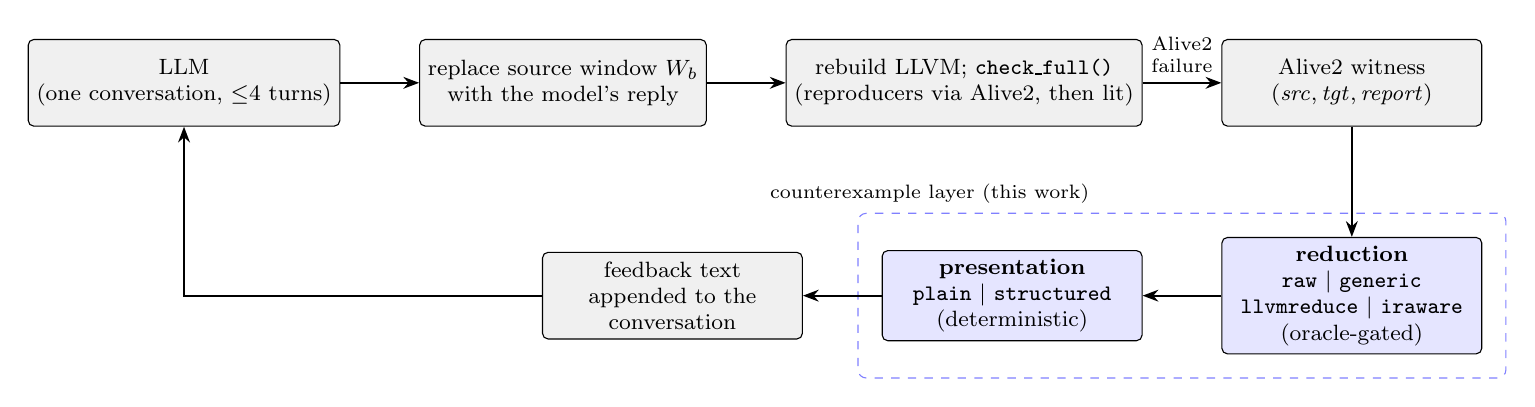
\begin{tikzpicture}[
  font=\footnotesize,
  box/.style={draw, rounded corners=2pt, align=center, minimum height=11mm, minimum width=33mm, inner sep=3pt},
  inh/.style={box, fill=black!6},
  ours/.style={box, fill=blue!10},
  arr/.style={-{Stealth[length=2mm]}, thick},
  lbl/.style={font=\scriptsize, align=center}]
\node[inh] (llm) {LLM\\(one conversation, $\le$4 turns)};
\node[inh, right=10mm of llm] (patch) {replace source window $W_b$\\with the model's reply};
\node[inh, right=10mm of patch] (check) {rebuild LLVM; \texttt{check\_full()}\\(reproducers via Alive2, then lit)};
\node[inh, right=10mm of check] (wit) {Alive2 witness\\$(\mathit{src},\mathit{tgt},\mathit{report})$};
\node[ours, below=14mm of wit] (red) {\textbf{reduction}\\\cn{raw} $\mid$ \cn{generic}\\\cn{llvmreduce} $\mid$ \cn{iraware}\\(oracle-gated)};
\node[ours, left=10mm of red] (pres) {\textbf{presentation}\\\cn{plain} $\mid$ \cn{structured}\\(deterministic)};
\node[inh, left=10mm of pres] (fb) {feedback text\\appended to the\\conversation};
\draw[arr] (llm) -- (patch);
\draw[arr] (patch) -- (check);
\draw[arr] (check) -- node[above, lbl]{Alive2\\failure} (wit);
\draw[arr] (wit) -- (red);
\draw[arr] (red) -- (pres);
\draw[arr] (pres) -- (fb);
\draw[arr] (fb.west) -| (llm.south);
\begin{scope}[on background layer]
\node[draw=blue!50, dashed, rounded corners=3pt, fit=(red)(pres), inner sep=3mm, label={[font=\scriptsize]above left:counterexample layer (this work)}] {};
\end{scope}
\end{tikzpicture}
\caption{The counterexample layer (blue) inside the adapted repair loop (grey). Reduction and presentation are separate factors. A passing check ends the run. Other failures (build, lit, unmatched window) bypass the layer. The \cn{baseline} condition substitutes a fixed sentence for an Alive2 counterexample. The initial prompt also includes feedback from the unpatched compiler.}
\label{fig:arch}
\end{figure*}

\subsection{The preserved property: the oracle}

Every reducer proposes a candidate pair and asks an oracle whether the violation survives. The oracle runs \texttt{alive-tv} on the candidate and compares the result with the violation reported for the original pair. That violation is described by the function name, the Alive2 error class (for example, ``Target is more poisonous than source''), and a coarse \emph{kind} of target-side outcome (poison, undef, UB, or a concrete wrong value) inferred from the report. Three strictness levels are defined:
\begin{itemize}
\item \cn{any\_failure}: some refinement failure is still reported, in any function;
\item \cn{error\_class} (the default): a failure with the same error class is reported in the same function;
\item \cn{error\_class\_and\_kind}: additionally, the target-side outcome kind matches.
\end{itemize}

A candidate that Alive2 cannot parse or type-check is rejected, as is a candidate whose run errors without reporting a violation. Matching an error class is weaker than preserving the original root cause or the original execution, because two different inputs or two different flags can trigger the same class in the same function. At \cn{any\_failure}, the reducer may drift onto an unrelated bug. A reduced witness is therefore a valid counterexample with the same error class in the same function. It is not a proof of equivalence with the original witness, and it is not guaranteed to be globally minimal.

\subsection{Baseline reducers}

\textbf{\cn{generic}.} The reduction units are the lines of both files. A variant of \texttt{ddmin} proposes subsets and complements, and each candidate is rendered by concatenating the surviving lines of each file. The reducer has no notion that the files are versions of one function, so candidates that contain lines from only one side are simply rejected. Relative to the original algorithm~\cite{zeller2002dd}, the implementation jumps directly to single-element granularity when no subset or complement succeeds, instead of doubling the number of chunks.

\textbf{\cn{llvmreduce}.} \texttt{llvm-reduce} accepts one file and one interestingness test, so the pairing is supplied from outside. The wrapper first reduces the source with the target held fixed. It then reduces the target with the \emph{already reduced} source held fixed, and finally it checks the reduced pair together. The tool's own passes are unmodified. Each candidate spawns a separate process that runs the oracle and returns only an exit status, so the tool never sees the violation or the other file. This isolates ``understands IR'' from ``understands the counterexample.''

\subsection{The IR-aware reducer}

The reducer operates on a parsed model of the module (Section~\ref{sec:impl}) rather than on text. It differs from the baselines in three ways.

\emph{Tandem editing.} Source and target are two versions of one function. Edits are applied to both and matched by SSA name, so that deleting a value on one side deletes the same-named value on the other.

\emph{Dependency-closed candidates.} Instead of deleting lines, the reducer chooses a set of values to \emph{keep}. It then closes this set over def-use edges, the operands of terminators and returns, and the branch conditions of every block from which the kept values are reachable. Everything outside the closure is removed. This avoids dangling uses by construction. It does not guarantee a valid module, because type or phi-edge inconsistencies and parser misreads remain possible, which is why every candidate still goes to the oracle.

\emph{Counterexample-derived seeds.} The verifier report provides three kinds of information. First, it supplies the \emph{seeds}, which are the values the reducer must keep: values whose trace values differ between source and target, values that are poison, undef, or UB on the target side, and values that appear only on the source side. The values returned by the source function are added to this set. Second, it records the \emph{executed blocks} on the source side, which determine the branch to fold. Third, it gives the \emph{type} of each value printed in the example and traces, which is used when a value is promoted to a parameter.

\begin{table}[t]
\caption{Passes of the IR-aware reducer, in application order. Every proposal is gated by the oracle.}
\label{tab:passes}
\centering\footnotesize
\begin{tabular}{@{}p{2.75cm}p{4.75cm}@{}}
\toprule
Pass & Proposal \\
\midrule
\cn{dce} & delete values that no instruction reads, except seeds (up to 16 sweeps) \\
\cn{fold-branches} & replace a conditional branch by an unconditional one to the successor that the source trace entered, when exactly one successor was entered \\
\cn{prune-blocks} & delete blocks unreachable from entry, pruning \texttt{phi} edges \\
\cn{simplify-cfg} & replace single-edge \texttt{phi}s by their value; splice a block into its sole unconditional predecessor (up to 32 steps) \\
\cn{slice} & pin the seeds; \texttt{ddmin} over the remaining source values, each subset closed as above and applied to both sides \\
\cn{promote-operands} & replace a non-seed, non-\texttt{phi} value defined on both sides by a fresh parameter of the trace's type, then delete dead producers \\
\cn{drop-params} & remove parameters unused on both sides \\
\cn{strip-flags} & \texttt{ddmin} over the \texttt{nsw}, \texttt{nuw}, \texttt{exact}, \texttt{inbounds}, \texttt{nneg}, \texttt{disjoint}, \texttt{samesign} and fast-math flags on either side \\
\bottomrule
\end{tabular}
\end{table}

Table~\ref{tab:passes} lists the passes, and Algorithm~\ref{alg:iraware} gives the driver. Branch folding is unsound in general (for instance, when the condition is poison), which is one reason the oracle gates it.

\textbf{Operand promotion generalizes the witness.} A fresh parameter may take any value of its type, so the reduced pair may describe an execution that the original program cannot reach. The oracle guarantees that the violation is preserved, but not that it remains relevant to the original bug. Promotion is therefore separately switchable (\texttt{--no-promotion}) and is the subject of the ablation in RQ6.

\begin{algorithm}[t]
\caption{IR-aware reduction (as implemented)}
\label{alg:iraware}
\begin{algorithmic}[1]
\Require $\mathit{src},\mathit{tgt}$, parsed violation $R$ (function $f$), oracle $\mathcal O$ with budget $B$, flag \textsc{promote}, $\mathit{max\_rounds}{=}4$
\State parse both modules; \textbf{if} parsing fails or $f$ is missing in either \textbf{return} unreduced with an error
\State $\mathit{seeds}\gets$ diverging, target-poison/undef/UB, and source-only trace values $\cup$ values returned by $f_{src}$
\State $\mathit{types}\gets$ value types in $R$;\; $\mathit{exec}\gets$ source-side blocks entered in $R$
\State $S\gets(f_{src},f_{tgt})$;\; $\mathit{applied}\gets\emptyset$
\For{$\mathit{round}=1$ \textbf{to} $\mathit{max\_rounds}$}
  \State $\mathit{progress}\gets\textbf{false}$
  \For{\textbf{each} pass $P$ \textbf{in} \cn{dce}, \cn{fold-branches}, \dots, \cn{strip-flags}}
    \If{$\mathcal O$.exhausted} \textbf{break} \EndIf
    \State $S'\gets P(S)$ \Comment{each accepted proposal: $\mathcal O(\textsc{render}(S'))$ preserves the violation}
    \If{$S'\neq\bot$} $S\gets S'$;\; $\mathit{applied}\gets\mathit{applied}\cup\{P\}$;\; $\mathit{progress}\gets\textbf{true}$ \EndIf
  \EndFor
  \If{\textbf{not} $\mathit{progress}$ \textbf{or} $\mathcal O$.exhausted} \textbf{break} \EndIf
\EndFor
\If{$\mathit{applied}\neq\emptyset$ \textbf{and not} $\mathcal O(\textsc{render}(S))$} \textbf{return} the original pair \EndIf
\State \Return $\textsc{render}(S)$
\end{algorithmic}
\end{algorithm}

\subsection{Presentation}

\textbf{Plain.} The text consists of ``Source:'' followed by the IR of the (possibly reduced) source, ``Target:'' followed by the target IR, and then Alive2's own report from the line ``Transformation doesn't verify!'' onward. The report includes the example input, the per-value traces for both sides, and the final values. When the pair was reduced, the report comes from re-running Alive2 on the reduced pair, so the trace describes the IR that is shown.

\textbf{Structured.} The same IR pair is shown, followed by labelled sections: bug type, verification result, violated property, a diff of source and target keyed by SSA name rather than by line, critical values (the seeds), the dependency chain of the seeds in the source, the blocks entered, the counterexample input, the first divergences between source and target values, memory state when present, and an interpretation. The interpretation is a fixed template per Alive2 error class, filled with values from the report. Six error classes have templates, and other classes receive a one-sentence fallback. A further sentence names any flag that is present in the target and absent in the source. No text is produced by a model. Structured presentation is not information-neutral. It omits the per-value traces that the plain report contains, and it adds derived sections (the diff, the dependency chain, and the interpretation). Differences between \cn{plain} and \cn{structured} are therefore differences in both organization and content.

\subsection{Fallbacks and stopping}

Reduction returns the unreduced pair when parsing fails, the named function is absent, or a final check fails. In the evaluated version, exhausting the 400-call reducer budget can itself cause the final check to fail and discard progress. The renderer separately re-verifies a changed pair before using its refreshed trace. That call is outside the reducer's 400-call counter, so this setting is not a bound on all verifier work in a repair run.

The IR-aware reducer stops after at most four rounds of the eight passes, when a round makes no progress, or when the budget is exhausted. It does not claim to reach a fixed point or a globally minimal witness. Within a pass, \texttt{ddmin} can reach a 1-minimal subset with respect to that pass's units if it is not interrupted. The \texttt{llvm-reduce} wrapper is additionally capped at 600~s of wall-clock time per side. Fallback causes and the size actually shown to the model must be inspected alongside accepted-pass counts.

%=====================================================================
\section{Implementation}
\label{sec:impl}
%=====================================================================

\subsection{Evaluated v2 implementation}

The implementation is the \texttt{ce} Python package and an adapted repair runner in the project repository~\cite{betterCompiler2026}. The evaluated harness is identified as \cn{repair-v2}; its code is anchored at commit \texttt{38b381b}. This draft uses the 205-record data snapshot at \texttt{73f2ba1} on branch \texttt{feat/h100-sweep}. Older Qwen2.5 runs, earlier Qwen3 runs, and the held-out development pilot are not pooled with it. The benchmark is a vendored copy of \emph{llvm-apr-benchmark} whose upstream commit is not recorded. The repository's build recipe pins Alive2 at \texttt{f9a4f02f}; the exact native binary and host package versions still require an environment capture from the H100 node.

\textbf{Alive2 interface and parser.} \texttt{alive-tv} is invoked with \texttt{--disable-undef-input}, as in the benchmark, after \texttt{noalias} and \texttt{nofree} are removed from both files (the benchmark's own pre-pass). The parser splits the output at the separator line and reads the error class from the \texttt{ERROR:} line. It also reads the example, the two traces (including the \texttt{Jump to} annotations), the source and target values, and the memory-state blocks. Alive2's output format is not a documented interface. Anything unrecognized stays in the raw text, and output with no parseable section is reported as a tool error.

\textbf{IR model.} The model is line-oriented and is not an LLVM parser. It separates the module preamble from function definitions and splits each function into parameters, blocks, and instructions, recording result names, opcodes, value operands, and label operands. Bracketed instructions that span several lines are joined. The repository's parse-and-print check preserves all 1{,}462 stored reproducer bodies after trailing newline characters are removed for comparison. This checks unchanged round trips, not the correctness of edits. Invalid candidates are normally rejected by the oracle, but error-class matching can still permit semantic drift. Source and target are paired by SSA name, which assumes corresponding values retain their names.

\textbf{Feedback assembly.} After checking the unpatched compiler, the runner processes its failure into the initial user prompt. Later failures are processed in the same way. The adapter selects the first failing test; an Alive2 report receives the selected reduction and presentation, while other diagnostics pass through with an effectively nonbinding $10^9$-character cap. In v2, the reduction oracle and trace refresh omit the per-test \texttt{additional\_args} used by the benchmark's original check. Five sampled bugs carry such arguments: 126012, 114879, 91369, 180870, and 91957. For these bugs, the reduced witness may be checked under different unrolling settings. These records are retained and flagged; a correction cannot retrospectively change the feedback that was shown.

\textbf{Repair loop.} The runner follows the benchmark's hint-based path. The system prompt asks for a small targeted LLVM repair that preserves unrelated optimizations and IR invariants. The first user turn states the bug type, primary component, issue title without its body, condition-specific feedback, and a C++ source window. The window comes from the first hinted file at the base commit, extends the hinted range by 30 lines on each side, and is expanded by a bounded brace-balancing heuristic. This heuristic is not a C++ parser and can still expose partial statements or functions.

In v2, the reply must contain the full replacement window, including requested prefixes and suffixes. Extracted code is substituted for the original window. Before every proposal, the tree is reset to the base commit, so replies are relative to the original source rather than the preceding patch. The conversation retains previous proposals and feedback. Whitespace-normalized unchanged replies consume a turn, receive a fixed corrective message, and bypass building. An unmatched window also consumes a turn without validation. Other replies are built and checked. The v2 extraction and full-window protocol can turn incomplete or poorly formatted replies into invalid C++; these failures remain part of its measured outcome.

\textbf{Model and serving.} We use \texttt{Qwen3-Coder-30B-A3B-Instruct}, a sparse model with 30.5B total and 3.3B activated parameters~\cite{qwen3coder30b}. The operator-reported server uses online FP8 quantization on an H100, vLLM 0.28.0, a 32{,}768-token maximum context, GPU-memory utilization 0.55, eager execution, and the FlashInfer sampler disabled. The client uses temperature 0.8 and a 300~s request timeout, with no explicit generation seed, \texttt{top\_p}, or completion-token limit. Effective server defaults and the exact checkpoint revision are not captured by the v2 manifest and remain to be archived. The manifest fixes the model alias, temperature, four-turn budget, oracle settings, prompt hash, and harness identifier. It therefore guards incompatible resumes but is not a complete model or toolchain provenance record.

\textbf{Version history.} Earlier full-window prompts and models produced many unchanged replies. V2 adds a no-op guard, the brace heuristic, and a stronger instruction to make a targeted edit; all nine conditions use these changes. The excluded bug 115575 was used for a nine-condition v2 pilot. It is a development check, not an additional evaluation bug. The original draft's 45 passing and 18 skipped tests describe an earlier source snapshot; those counts do not certify the current native experiment.

\subsection{Revised v3 implementation awaiting evaluation}

A revised v3 implementation forwards per-test verifier arguments, uses strict response parsing and atomic search/replace edits, rejects length-truncated completions, and sets an 8{,}192-token output limit. It also avoids unconsumed terminal feedback, caches previously verified candidate pairs, reserves a final validation call for LLVM-reduce, checks the refreshed failure class, and records the witness actually shown after fallback. These changes affect the edit interface and feedback semantics. They require a fresh output directory and H100 validation on development inputs. No v3 repair outcomes are reported here, and v2 and v3 records will not be pooled. Section~\ref{sec:v3} specifies the amended follow-up.

%=====================================================================
\section{Experimental Design and Evaluation Protocol}
\label{sec:design}
%=====================================================================

The original main protocol specifies 24 bugs, three trials, and nine conditions. This draft audits a frozen partial v2 snapshot and describes a separate v3 follow-up. A repository document dated 2026-09-04 specifies the repeat count, test, and four primary comparisons before the repair records it describes. This is a record in repository history, not an external preregistration. Later model and harness changes are disclosed in a dated amendment. The v3 follow-up is fixed before observing its outcomes, but it is not a completion of the original unchanged protocol.

\subsection{Population}

\begin{table}[t]
\caption{From the full benchmark to the sample, counted from the vendored dataset files.}
\label{tab:funnel}
\centering\footnotesize
\begin{tabular}{@{}p{6.4cm}r@{}}
\toprule
Stage & Bugs \\
\midrule
Dataset files (crash 340, miscompilation 142, hang 9) & 491 \\
Miscompilations checked with Alive2 (7 are \texttt{lli}-only) & 135 \\
\ldots\ with \texttt{is\_single\_func\_fix} (eligible subset) & 100 \\
\ldots\ minus bootstrap bug 115575 (sampling pool) & 99 \\
Sample: 8 per tier, tiers of 33 & 24 \\
Interim complete panel (3 trials, all 9 conditions) & 7 \\
\bottomrule
\end{tabular}
\end{table}

A bug is eligible if it is a miscompilation, every reproducer is checked by Alive2 rather than \texttt{lli}, and the reference fix touches one function. The counterexample conditions require the first filter, and the runner skips multi-function fixes. The pool excludes bug 115575, which was used during harness development. The pool is sorted by hint-region size (the number of lines covered by the bug-location hints), then by reproducer size, then by identifier, and it is cut into three tiers of 33 bugs. Within each tier, bugs are drawn round-robin across the first hinted component, so that InstCombine (45 of the 100 eligible bugs) does not dominate. The procedure is deterministic, and re-running the selection script reproduces the committed list. The tier labels in the repository (easy, medium, hard) describe the size of the hint region and reproducer, not measured difficulty for any model.

The sample has 16 distinct primary component labels, one of which is a placeholder for a bug with no component hint. Eleven of the 24 bugs have knowledge cutoffs in 2025 or 2026. Results will be reported over this subset of miscompilations only, not over the whole benchmark. The runner additionally skips a bug whose failure does not reproduce at its base commit, so the analyzed count may be below 24.

\subsection{Conditions}

\begin{table}[t]
\caption{The nine conditions. The \cn{baseline} condition receives a fixed sentence and no counterexample.}
\label{tab:conditions}
\centering\footnotesize
\begin{tabular}{@{}lll@{}}
\toprule
Reduction & \cn{plain} & \cn{structured} \\
\midrule
(none) & \cn{baseline} & --- \\
\cn{raw} & \cn{raw-plain} & \cn{raw-structured} \\
\cn{generic} & \cn{generic-plain} & \cn{generic-structured} \\
\cn{llvmreduce} & \cn{llvmreduce-plain} & \cn{llvmreduce-structured} \\
\cn{iraware} & \cn{iraware-plain} & \cn{iraware-structured} \\
\bottomrule
\end{tabular}
\end{table}

\textbf{Held constant.} Within v2, every condition uses the same model, prompt template apart from feedback, source window, four-turn limit, oracle budget of 400, \cn{error\_class} strictness, and temperature. Feedback length and content differ by design. Other failure types follow the same handling policy, although their diagnostic text varies with each proposal. Earlier Alive2 evidence remains in the conversation during later build or lit failures. LLM sampling is not seeded.

\subsection{Procedure and budget}

The main design contains 648 runs: 24 bugs by 9 conditions by 3 trials. The planned promotion-disabled ablation adds 144 runs and is not yet available in this snapshot. A run permits four model replies; unchanged or unapplied replies bypass building, applied replies reach the build stage, and lit runs only after the reproducers pass. The runner uses bug-major order to reuse incremental builds and compiler caches. The reported build concurrency is 64 jobs; compilation and lit run on CPUs rather than the H100 inference device.

Records are written atomically. Resume skips a valid completed run: an early success, or a run that exhausted its reply budget without an endpoint-error flag. Endpoint failure before the first reply leaves the cell empty; later endpoint failures are flagged and treated as incomplete on resume. Failed unpatched builds stop the sweep as setup failures. Final comparisons require the same bugs and all three completed trials per compared condition; missing or infrastructure-interrupted cells are not silently treated as model failures.

\subsection{Success criterion}
\label{sec:success}

A run succeeds on the first turn at which the benchmark's \texttt{check\_full()} returns true. That function performs three steps. (i) It builds LLVM with CMake and Ninja in \texttt{RelWithDebInfo} mode with assertions enabled, for the X86, RISCV, AArch64, SystemZ, Hexagon, PowerPC, and NVPTX targets. (ii) It runs every reproducer test through \texttt{opt} and requires Alive2 to report zero incorrect transformations, zero failed-to-prove transformations, and zero errors. (iii) It checks out the \texttt{llvm/test} tree of the fix commit and runs \texttt{llvm-lit} over the directories listed for that bug (one directory for 23 of the 24 sampled bugs and four for bug 114879), stopping at the first failure, with a 300~s limit.

This is a plausibility criterion, bounded by Alive2's unroll limit and by the listed test directories. It is not a proof of correctness and does not cover the whole LLVM regression suite. Because the \emph{llvm-harness} expert review found benchmark-passing patches that were invalid~\cite{zheng2026harness}, we call a passing patch \emph{plausible}. Manual assessment of the candidate's semantics and optimization preservation remains necessary before describing a harness pass as a confirmed correct repair.

\subsection{Metrics}

The primary outcome is the bug-level success indicator \emph{pass@3}: a bug counts as repaired under a condition if at least one of its three completed trials succeeds. Here pass@3 denotes this observed per-bug indicator. When all three trials of a cell exist, it coincides with the unbiased pass@$k$ estimator for $n=k=3$~\cite{yang2026reducefix}, but it is not an estimate from a larger sample. \emph{Pass@1}, the fraction of individual runs that succeed, is reported alongside it. One run permits four replies, so pass@1 is not a first-reply success rate. The bug is the unit of analysis: repeated trials do not add independent bugs. Interim repair comparisons use the common panel with all three trials under every condition. The secondary measures are as follows.
\begin{itemize}
\item Iterations to repair (LLM turns until success) and the build and verifier-call counts that scale with it. Runs that do not succeed are censored at the iteration limit, so the repository's unconditional mean is not by itself an efficiency estimate. The analysis of this measure is not specified in the repository.
\item Reducer measures: instructions, lines, blocks, values, and characters in the witness actually shown; oracle calls; accepted and rejected candidates; tool failures; and seconds. Accepted-pass names alone do not establish size reduction.
\item LLM prompt and completion tokens as reported by the server, and an \emph{estimated} feedback size (characters divided by four), which is used only to compare conditions.
\item Recorded wall-clock time, which is descriptive. V2 still constructs feedback after the final failed reply, although no model turn consumes it. Per-turn feedback totals omit this terminal work and may undercount oracle activity.
\end{itemize}

\subsection{Inference}

Four comparisons are primary, each in a direction stated beforehand: \cn{iraware-plain} versus \cn{generic-plain}, \cn{iraware-plain} versus \cn{llvmreduce-plain}, \cn{iraware-structured} versus \cn{iraware-plain}, and \cn{raw-plain} versus \cn{baseline}. For a pair, let $b$ be the number of bugs repaired only under the hypothesized-better condition and $c$ the number repaired only under the other. The exact one-sided McNemar test conditions on $n=b+c$ and uses the binomial tail
\begin{equation}
p=\sum_{i=b}^{n}\binom{n}{i}2^{-n}.
\end{equation}
The four $p$-values are adjusted together with the Benjamini--Hochberg procedure~\cite{benjamini1995fdr} at $\alpha=0.05$. For every comparison, the analysis script also prints the repaired counts, $b$, $c$, the paired difference in proportions, an odds ratio, and a two-sided $p$-value. We report $b$, $c$, and the difference regardless of the $p$-value, and we do not read a non-significant result as evidence of no effect. The other 32 pairs are exploratory and are reported uncorrected and descriptively. The ablation compares each \cn{iraware} condition with itself under promotion on and off, as a separate family of two tests. The script tests the one-sided hypothesis that promotion on is better, so a benefit of disabling promotion would not be detected by that test.

Fewer than five discordant bugs cannot yield $p<0.05$ one-sided at any split, and $n=24$ limits power. Under assumed per-attempt rates of 0.12--0.35 and a per-bug difficulty multiplier, the repository's simulation gives power between roughly 0.10 and 0.57 at three trials. The assumptions are the authors' and are based on reported frontier-agent rates rather than on data from this setup. The comparison is therefore best read as a pilot-scale screen. Conditions should have equal numbers of trials before pass@3 is compared.

\subsection{Dated amendment: prospective v3 follow-up}
\label{sec:v3}

After the v2 audit, an amendment dated 2026-10-22 assigns the original 16 medium- and hard-tier bugs to a separate v3 evaluation. The eight first-tier bugs informed v2 harness debugging and are excluded from that follow-up. The remaining tiers are not a pristine held-out set: bug 115149 was previously used in earlier Qwen3 diagnostics and known-patch validation. The follow-up is prospective with respect to v3 outcomes, not the authors' first exposure to every bug. The source manifest \texttt{data/repair\_v3\_protocol.json} fixes the identifiers, condition set, and budgets before v3 repair outcomes are collected.

To fit the remaining computation budget, the follow-up uses six conditions: \cn{baseline}, \cn{raw-plain}, \cn{generic-plain}, \cn{llvmreduce-plain}, \cn{iraware-plain}, and \cn{iraware-structured}. These retain all four original primary comparisons. Three trials and four replies per run give 16 by 6 by 3 = 288 planned runs. The same generation and validation settings are applied across those conditions, with the v3 changes described above. This subset does not retain the full factorial design, so it cannot estimate every reduction--presentation interaction. No v3 outcome or promotion-off result is available in this draft.

The amendment separates development observations from prospective follow-up data, rather than pooling them into a larger apparent sample. It also reduces the paired sample from 24 to 16; statistical significance is therefore not assured. The hypothesis directions, four-comparison correction family, matched-trial rule, and plausibility criterion remain unchanged. Any secondary-model pilot on the excluded development bug would be a feasibility check and would not contribute to the v3 outcome table.

For v3, candidate-oracle calls and separate trace-refresh calls will be reported individually and together as feedback-verification work. That sum still excludes the benchmark's reproducer and regression-validation work. This avoids treating the 400-call candidate budget as a complete verifier-cost measurement.

%=====================================================================
\section{Results}
%=====================================================================

\subsection{Snapshot coverage}

The frozen v2 snapshot contains 205 runs over eight observed bugs. It has ten full-validation passes across three bugs: 89390, 135182, and 126012. The eighth bug, 126012, has not completed all trials and conditions. It is included in the diagnostic totals but excluded from the matched repair table. Seven bugs form the complete panel, with 189 runs and 21 trials per condition. All seven belong to the first size tier, so this panel does not represent the planned 24-bug sample's balance. These are preliminary descriptive results, not a final significance analysis.

% Generated by scripts/report_snapshot.py; edit the generator rather than these values.
% Snapshot 73f2ba151742c44cf88878b50c027ef7f06293c6
\begin{table}[t]
\centering\scriptsize
\caption{Diagnostic v2 outcomes on 7 fully matched bugs (three trials each). These are harness-passing outcomes, not expert-certified repairs. Incomplete bugs are excluded.}
\label{tab:v2-matched}
\begin{tabular}{@{}lrr@{}}\toprule
Condition & Bugs / 7 & Runs / 21 \\ \midrule
\texttt{baseline} & 0 & 0 \\
\texttt{raw-plain} & 0 & 0 \\
\texttt{raw-structured} & 2 & 4 \\
\texttt{generic-plain} & 1 & 1 \\
\texttt{generic-structured} & 0 & 0 \\
\texttt{llvmreduce-plain} & 1 & 2 \\
\texttt{llvmreduce-structured} & 1 & 1 \\
\texttt{iraware-plain} & 1 & 1 \\
\texttt{iraware-structured} & 0 & 0 \\
\bottomrule\end{tabular}
\end{table}
\begin{table}[t]
\centering\scriptsize
\caption{Descriptive paired counts for the four prespecified comparisons on 7 complete bugs. $b$ favors the hypothesized direction, $c$ opposes it. P1: IR-aware vs generic; P2: IR-aware vs llvm-reduce (both plain); P3: IR-aware structured vs plain; P4: raw plain vs baseline. This interim snapshot is not a significance-based stopping analysis.}
\label{tab:v2-pairs}
\begin{tabular}{@{}lrrrrr@{}}\toprule
Pair & Both & $b$ & $c$ & Neither & $p_{\rm BH}$ \\ \midrule
P1 & 0 & 1 & 1 & 5 & 1.000 \\
P2 & 1 & 0 & 0 & 6 & 1.000 \\
P3 & 0 & 0 & 1 & 6 & 1.000 \\
P4 & 0 & 0 & 0 & 7 & 1.000 \\
\bottomrule\end{tabular}
\end{table}
\begin{table}[t]
\centering\scriptsize
\caption{Turn diagnostics over all 205 saved runs, including incomplete bugs. Categories are mutually exclusive validation endpoints; parser and linker symptoms are diagnostic subsets, not model-correctness judgments.}
\label{tab:v2-diagnostics}
\begin{tabular}{@{}lr@{}}\toprule
Measure & Count \\ \midrule
Model turns & 810 \\
Applied proposals reaching a build & 723 \\
Build-stage failures & 467 \\
Reproducer-stage failures & 205 \\
Regression-stage failures & 41 \\
Full-validation passes & 10 \\
Unchanged proposals & 87 \\
Build failures with fence contamination & 71 \\
Build failures with undefined symbols & 124 \\
\bottomrule\end{tabular}
\end{table}
\begin{table}[t]
\centering\scriptsize
\caption{Initial witness instruction counts from trial 1 of each plain condition, over 8 observed bugs. $I_0$: original; G: generic; L: llvm-reduce; A: IR-aware. Counts alone do not establish preservation of the original bug or repair usefulness.}
\label{tab:v2-reducers}
\begin{tabular}{@{}lrrrr@{}}\toprule
Bug & $I_0$ & G & L & A \\ \midrule
89390 & 8 & 8 & 3 & 8 \\
165878 & 19 & 19 & 3 & 19 \\
135182 & 10 & 10 & 2 & 10 \\
126974 & 10 & 10 & 10 & 4 \\
154116 & 8 & 8 & 5 & 8 \\
116249 & 21 & 21 & 2 & 18 \\
143123 & 6 & 6 & 4 & 6 \\
126012 & 27 & 27 & 27 & 27 \\
\bottomrule\end{tabular}
\end{table}


\subsection{Matched repair outcomes}

Table~\ref{tab:v2-matched} reports the common panel. Raw structured feedback repairs two of seven bugs, while generic plain, LLVM-reduce plain, LLVM-reduce structured, and IR-aware plain each repair one. IR-aware structured, raw plain, generic structured, and the no-counterexample baseline repair none. The successful bugs in this panel are 89390 and 135182. These counts do not show that IR-aware reduction improves repair.

The primary paired counts are given in Table~\ref{tab:v2-pairs}. IR-aware plain and generic plain each repair a different bug, giving $b=c=1$. IR-aware plain and LLVM-reduce plain repair the same bug, giving no discordant pairs. The structured IR-aware condition has one loss and no exclusive success relative to IR-aware plain. Raw plain and the baseline both have zero successes. All four BH-adjusted $p$-values are 1.0. With at most two discordant bugs, these comparisons provide little information about an effect. The larger count for raw structured feedback is exploratory and does not establish superiority.

\subsection{Failures and treatment delivery}

Across all 205 records, 810 model replies were recorded. Of these, 87 return unchanged code and 723 reach a build; 467 build attempts fail. Saved diagnostics include stray backticks, undeclared names, missing or incompatible LLVM APIs, and linking errors. A build-stage label alone cannot attribute the failure to hardware or to model reasoning. The source and reply audit identifies failures in the full-window and code-fence protocol, so the compilation rate is partly a property of this harness version. Other failures remain candidate-code errors. Table~\ref{tab:v2-diagnostics} keeps these stages separate.

Ten turns pass full validation and 41 reach regression testing but fail there. Certificate flags record whether any turn passed the reproducer, and are not statements about the final saved patch. Case studies must therefore use the corresponding reply rather than a later failed proposal. Regression failures include optimization expectations in VectorCombine and InstCombine; passing a reproducer alone is not enough.

Offline inspection also limits the interpretation of the ten passing patches. For bug 89390, two LLVM-reduce-condition proposals disable the affected folding step for every integer division or remainder operation. The reference fix instead guards those operations when the shuffle mask contains poison. The proposals may therefore sacrifice valid optimizations even though the selected checks pass; the performance effect has not been measured. We retain their harness-pass labels and do not treat source differences alone as proof of incorrectness. Correctness and optimization-preservation review remain pending.

Table~\ref{tab:v2-reducers} summarizes the first initial witness per observed bug. The audit also finds no accepted IR-aware reduction on any recorded witness for 89390, 135182, and 126012. These are the same three bugs with full passes somewhere in the snapshot. Thus a passing repair in an IR-aware condition cannot, by itself, be attributed to successful IR-aware shrinking. An unchanged witness can still receive structured presentation, and stochastic generations can differ even when feedback is identical. The promotion-disabled ablation and the remaining size tiers are not yet evaluated.

%=====================================================================
\section{Discussion}
%=====================================================================

The preliminary snapshot shows that the model can produce plausible LLVM repairs, but it does not show an advantage for the proposed reducer. The condition with the most repaired bugs is raw structured feedback, and its advantage is only two bugs in a seven-bug panel. The absence of passes under the no-counterexample baseline and raw plain feedback also leaves the anchor comparison without discordant outcomes. These results should guide an implementation audit, not a new claim of statistical significance.

The main practical limitation is the number of turns that fail before semantic validation. Improving response parsing and the edit interface may recover useful repair attempts, but it would change the harness. Any resulting gain must first be described as a gain from the revised repair procedure. Evidence for the counterexample method would still require comparing its feedback conditions within that revised procedure. Mixing revised runs into v2 would confound the two changes.

Reducer behavior also needs to be separated from repair success. Some initial witnesses are already short, while budget fallbacks or missing verifier arguments can prevent useful edits. The three bugs repaired somewhere in this snapshot have no accepted IR-aware reduction in their recorded feedback. This observation limits attribution, but does not establish that reduction is ineffective on the larger witnesses outside this v2 snapshot. Evaluating the remaining tiers, inspecting actual shown sizes, and examining fallback causes are needed to address that question.

A useful final analysis should examine whether reduced feedback changes the repairs proposed, whether those repairs preserve existing optimization behavior, and whether any improvement persists without operand promotion. All passing candidate patches should be reviewed before making a claim about correct repairs. Where the evidence remains inconclusive, the paper will report the measured counts and limitations rather than infer equivalence.

%=====================================================================
\section{Threats to Validity and Limitations}
\label{sec:threats}
%=====================================================================

The interim audit exposes implementation and coverage limits in addition to the design limitations below. Their effects cannot be cleanly separated from model capability in the present snapshot.

\textbf{Witness generalization.} Operand promotion can yield witnesses that describe unreachable executions. Only the ablation addresses this, and only through repair outcomes rather than through judgments of relevance.

\textbf{What the oracle preserves.} Equal error class in the same function does not imply equal root cause. The default strictness level was chosen as a compromise, results at other levels are not comparable, and only one level is planned.

\textbf{Bounded verification.} A reduced witness is a counterexample under the same bounded semantics, and the oracle cannot detect violations that require more loop iterations than Alive2's unroll bound. The omitted \texttt{additional\_args} on five sampled bugs (Section~\ref{sec:impl}) is a specific instance of this limitation in the present snapshot.

\textbf{Parser and model coverage.} The IR model is line-oriented, and the round-trip check does not test edits. When a parser error produces invalid IR or destroys the preserved violation, the oracle rejects the candidate, which typically turns the error into a missed reduction. However, because the oracle preserves an error class rather than semantic equivalence to the original witness, undetected semantic drift remains possible. Missed reductions make \cn{iraware} resemble \cn{raw} on the affected bugs. Unreduced fallbacks will be counted in the results.

\textbf{Reduction failures and budget.} A reduction that exhausts the budget is discarded rather than returned, so a tight budget biases the outcome toward unreduced witnesses. The budget of 400 calls is shared by the reducers in different ways: the \texttt{llvm-reduce} wrapper counts its subprocess calls against the same budget and additionally has a wall-clock cap that the other reducers lack.

\textbf{Source and target name matching.} Tandem editing and the structured diff assume that names correspond between the reproducer and the IR printed by the patched \texttt{opt}. Renumbered unnamed values or renamed instructions would appear as unrelated additions and removals. Only the target function with the reported name is reduced, and other functions in the module are left untouched.

\textbf{Prompt length and content.} Conditions differ in prompt length by construction. The \cn{generic} condition controls for length only if it actually shortens the prompt. The interim size measurements describe only the observed initial witnesses and do not establish the behavior on the remaining sample. In addition, \cn{structured} changes content as well as layout. Length is estimated as characters divided by four.

\textbf{Treatment reach.} Initial Alive2 feedback and later refinement failures are treated. Build and lit diagnostics are passed through without a useful length cap; they can dominate later conversation context. A compilation-failure turn still retains the earlier treatment in its history.

\textbf{Model dependence and sampling.} V2 uses one Qwen model and temperature 0.8. The client does not set \texttt{top\_p} or an output limit, and the exact checkpoint and server defaults remain to be archived. The effect may depend on model scale and training; three trials do not remove generation noise.

\textbf{Benchmark contamination.} The sampled bugs date from 2024-02 to 2026-02, so a model trained afterward may have seen the fixes. The harness records a self-declared model cutoff date that it does not verify, and we therefore make no claim about contamination-free evaluation. Contamination affects all conditions for a given bug, but it could produce a ceiling at which no condition is discordant.

\textbf{Localization hints.} The window is built from the benchmark's bug-location hints, which the benchmark describes as best-effort and which appear to be derived from the reference fix. The prompt also includes the issue title, which for some sampled bugs names the faulty flag or pass. The experiment therefore measures repair given a localized window, not autonomous localization. The brace-balancing heuristic does not guarantee statement or function boundaries, so a model can receive a partial function even in v2.

\textbf{Validation scope.} The \texttt{check\_full()} function bounds success as described in Section~\ref{sec:success}, and the Alive2 check passes only on the reproducers that the benchmark lists. A patch can be plausible and still incorrect, as the \emph{llvm-harness} review found in its own setting~\cite{zheng2026harness}.

\textbf{Departures from the inherited loop.} The runner differs from the benchmark's example loop (Section~\ref{sec:impl}). In particular, the \cn{raw-plain} condition does not reproduce the benchmark's prompt exactly, and the resulting rates are not comparable to published rates for the benchmark.

\textbf{Naming effects.} The reducer introduces parameter names of the form \texttt{\%ce.argN}. We know of no evidence on the effect of such names on models for IR. Evidence from Java repair shows sensitivity to renaming for fine-tuned models~\cite{rabbi2026hej}, but it need not transfer to this setting.

\textbf{Statistical resolution.} With 24 bugs, a non-significant comparison is uninformative about the absence of an effect. Pass@3 and pass@1 can disagree, and iterations to repair are conditional on repair. The contrast of the full method (\cn{iraware-structured}) against \cn{baseline} is not in the primary family and is exploratory.

\textbf{Scope and interim coverage.} The observed complete panel contains only seven first-tier bugs, rather than the planned 24. Findings concern single-function miscompilations checked by Alive2. They do not extend to crashes, hangs, multi-function fixes, or miscompilations checked by execution. V3 follows a data-informed harness revision and evaluates the original two remaining size tiers. Earlier exposure to bug 115149 is disclosed; prospective collection does not imply an untouched development set. V3 requires separate records and cannot erase the v2 findings.

%=====================================================================
\section{Conclusion}
%=====================================================================

We implemented a feedback layer that reduces and structures Alive2 counterexamples for localized LLVM repair. Its design separates reduction from presentation and preserves a selected failure class through a verifier oracle. The interim v2 evaluation contains 205 runs, but only seven bugs have complete three-trial coverage under every condition. These data show plausible repairs and substantial compilation failures; they do not establish that IR-aware reduction improves repair. The audit motivates a separate harness revision and further evaluation. The final result must depend on matched outcomes and reviewed patches, with the original primary comparisons and all protocol changes reported.

\bibliographystyle{IEEEtran}
\bibliography{references}

\end{document}
